% This is a copy version from https://github.com/thanhhungqb/thesis-template
% Please do not modified this project, when you want to start writing, make a clone of it for your own (Please read README.md)

\documentclass[12pt,a4paper,oneside]{book} % twoside for draf

%\usepackage{babel}
\usepackage[utf8]{vietnam}
\usepackage[utf8]{inputenc}
\usepackage{tipa}
\usepackage{amssymb}
\usepackage{graphicx}
\usepackage{subcaption}
\usepackage{booktabs}
\usepackage{mathptmx}	% same Time New Roma
\usepackage{amsmath}
\usepackage{amssymb}
\usepackage{amsfonts}
\usepackage{styles/ipa}
%\renewcommand{\rmdefault}{phv} % Arial
%\renewcommand{\sfdefault}{phv} % Arial
\usepackage{array}
\newcolumntype{P}[1]{>{\centering\arraybackslash}p{#1}}
\newcolumntype{M}[1]{>{\centering\arraybackslash}m{#1}}
\usepackage{fancyhdr}
\usepackage{multirow}
\usepackage{algorithm2e}
% Đổi tên mặc định của algorithm thành giải thuật nếu là 1, Các giải thuật nếu nhiều, Danh sách giải thuật nếu là ds
\SetAlgorithmName{Giải thuật}{Các giải thuật}{Danh sách giải thuật}
\usepackage{hyperref} % Hỗ trợ tạo hyperlink trong văn bản
\usepackage{float} % Hỗ trợ đặt hình ảnh chính xác

\linespread{1.25} % Giãn dòng 1.25 lần
% Set paragraph spacing
\setlength{\parskip}{\baselineskip}% Có nghĩa là khoảng cách giữa các đoạn là 1 dòng
% Load the parskip package with skip and indent options
\usepackage[skip=10pt plus1pt, indent=15 pt]{parskip} % Có nghĩa là khoảng cách giữa các đoạn là 10pt, và lùi đầu dòng 15pt
\usepackage{colortbl} % Hỗ trợ tạo bảng màu, VD: \cellcolor{gray} 

% \usepackage{algorithm}
% \usepackage{minted}
% \usepackage{minted}
\usepackage{listings}
\lstset{
  numbers=left,
  commentstyle=\color{green},
  keywordstyle=\color{blue},
  stringstyle=\color{red},
  basicstyle=\ttfamily,
  columns=flexible,
  breaklines=true
}
\usepackage{styles/cover}

\usepackage{graphicx}
\graphicspath{ {image/} }
\setcounter{secnumdepth}{2}
\crname{LUẬN VĂN TỐT NGHIỆP ĐẠI HỌC}
\ctname{NHẬN DIỆN VẬT THỂ TRONG ẢNH\\NHẬN DIỆN HƯỚNG NHÌN TRONG ẢNH}
\cstuname{
SVTH: NGÔ THỊ TIẾN (1413986)
}

\csCouncil{KHOA HỌC MÁY TÍNH}
\csReviewer{TS. TRẦN GIANG SƠN}
\csSupervise{TS. NGUYỄN ĐỨC DŨNG}
\cttime{12/2018}

\thesislayout

\begin{document}
%-	Bìa cứng - màu xanh dương, chữ mạ vàng (xem mẫu đính kèm)
%-	Trang tên (tờ lót): chất liệu giấy, nội dung giống như bìa LV
%-	Ở gáy LV: in nhan đề LV (có thể in tóm tắt nếu nhan đề quá dài), size 15 – 17
%-	Phiếu Nhiệm vụ LV, chấm điểm Hướng dẫn & Phản biện (đã ký): nhận từ GVHD & GVPB sau khi bảo vệ (theo lịch hẹn).
%-	Lời cam đoan
%-	Lời cảm ơn/ Lời ngỏ
%-	Tóm tắt LV
%-	Mục lục
%-	Danh mục, bảng biểu, hình ảnh, ... (nếu có)
%-	Nội dung LV
%-	Danh mục TL tham khảo
%-	Phụ lục (nếu có)

\coverpage

\frontmatter


\begin{declaration}
	Nhận diện hướng nhìn trong ảnh (Nhận diện vật thể trong ảnh) không phải là một đề tài mới nhưng vẫn là một thách thức bởi: trong các ứng dụng: việc nhận diện hướng nhìn của con người qua hình ảnh đòi hỏi kết quả chính xác cao, ở Việt Nam, hiện tại không  thực sự có nhiều nghiên cứu chuyên sâu về đề tài. Trong quá trình nghiên cứu đề tài có rất nhiều kiến thức không nằm trong chương trình giảng dạy ở bậc Đại học tuy vậy chúng tôi xin cam đoan đây là công trình nghiên cứu của riêng tôi dưới sự hướng dẫn của tiến sĩ Nguyễn Đức Dũng. Nội dung nghiên cứu và các kết quả đều là trung thực và chưa từng được công bố trước đây. Các số liệu được sử dụng cho quá trình phân tích, nhận xét được chính tôi thu thập từ nhiều nguồn khác nhau và sẽ được ghi rõ trong phần tài liệu tham khảo.

	Ngoài ra, tôi cũng có sử dụng một số nhận xét, đánh giá và số liệu của các tác giả khác, cơ quan tổ chức khác. Tất cả đều có trích dẫn và chú thích nguồn gốc.

	Nếu phát hiện có bất kì sự gian lận nào, tôi xin hoàn toàn chịu trách nhiệm về nội dung luận văn của mình. Trường đại học Bách Khoa thành phố Hồ Chí Minh không liên quan đến những vi phạm tác quyền, bản quyền do tôi gây ra trong quá trình thực hiện.

\end{declaration}

\begin{acknowledgments}

	Để hoàn thành kì đề cương luận văn này, tôi tỏ lòng biết ơn sâu sắc đến tiến sĩ Nguyễn Đức Dũng đã hướng dẫn tận tình trong suốt quá trình nghiên cứu.

	Chúng tôi chân thành cám ơn quý thầy, cô trong khoa Khoa Học Và Kỹ Thuật Máy Tính, trường đại học Bách Khoa thành phố Hồ Chí Minh đã tận tình truyền đạt kiến thức trong những năm chúng tôi học tập ở trường. Với vốn kiến thức tích lũy được trong suốt quá trình học tập không chỉ là nền tảng cho quá trình nghiên cứu mà còn là hành trang để bước vào đời một cách tự tin.

	Cuối cùng, tôi xin chúc quý thầy, cô dồi dào sức khỏe và thành công trong sự nghiệp cao quý.

\end{acknowledgments}

\begin{abstract}
	Nội dung chính của luận văn nhằm tìm hiểu, nghiên cứu xây dựng hệ thống nhận diện hướng nhìn thông qua ảnh chụp dựa trên những công trình, công nghệ mới được nghiên cứu và phát triển trong những năm gần đây của lĩnh vực Deep Learning. Trong quá trình nghiên cứu, tôi đã  tiến hành tổng hợp, đánh giá ưu và nhược điểm của cách phương pháp, công nghệ đã và đang được nghiên cứu, sử dụng. Tiếp cận vấn đề theo nhiều hướng khác nhau, tôi thực hiện một số phương pháp sử dụng học sâu (CNN) để phát hiện hướng nhìn của con người qua hình ảnh. Bên cạnh việc hoàn thành nội dung của đề tài, nhóm chúng tôi đã nghiên cứu thêm một số phần để từ đó đặt nền móng cho các nghiên cứu sau này. Phần còn lại của luận văn tập trung vào việc đánh giá mô hình, kết quả đạt được, đồng thời phân tích ưu nhược điểm của mô hình thực hiện và thảo luận những vấn đề mà mô hình còn gặp phải. Cuối cùng, nhóm chúng tôi đề xuất hướng phát triển tiếp theo của đề tài trong tương lai.
\end{abstract}


\tableofcontents
%\listofsymbols
% \listoftables
\listoffigures
%\listofalgorithms


\mainmatter

\fancyhead{}  % Clears all page headers and footers
%\rhead{\thepage}  % Sets the right side header to show the page number
%\lhead{}  % Clears the left side page header
%\fancyfoot[positions]{footer}
\renewcommand{\footrulewidth}{0.4pt}

\pagestyle{fancy}  % Finally, use the "fancy" page style to implement the FancyHdr headers
%
\chapter {Giới thiệu}

\section{Giới thiệu đề tài}
Sự tương tác giữa con người và máy tính ngày càng trở nên quan trọng khi các thiết bị thông minh như điện thoại, máy tính, máy tính bảng ngày càng gia tăng. Khoa học nghiên cứu về nó cũng được chú trọng phát triển theo, trong đó việc phát hiện hướng nhìn của người dùng thông qua đôi mắt trở thành một lĩnh vực trong thị giác máy tính ngày nay.

Qua các hình ảnh thu thập bằng máy quay trên thiết bị thông minh như điện thoại hay máy tính, ta có thể phát hiện được mục tiêu hay đối tượng mà người dùng đang hướng tới màn hình. Ứng dụng này có thể giúp người khuyết tật điều khiển các thiết bị chỉ bằng ánh mắt mà không cần đến đôi tay.

Tương tự như vậy khi gắn một máy quay nhỏ trên xe hơi theo dõi người lái xe, dựa vào hướng nhìn đôi mắt của tài xế mà ta có thể phát hiện kịp thời người này ngủ gật hay không chú ý khi lái xe (khi  ngủ gật mắt sẽ trùng xuống, khi không tập trung mắt sẽ hướng đi nơi khác).

Trong một lớp học hay một buổi dự thảo ta có thể đo được độ tập trung của người tham gia để kịp thời thay đổi nội dung cho phù hợp hơn, tránh lãng phí thời gian của mọi người.

Ngoài ra, việc dự đoán chính xác hướng nhìn của đôi mắt có thể phân tích hành vi mua hàng của khách như khách hay tập trung vào tầm nhìn nào nhiều nhất mà ta có thể sắp xếp mặt hàng quan trọng vừa tầm. Hay đơn giản như việc lướt web của người dùng Internet để sắp xếp nội dung quan trọng hay không quan trọng vào các vị trí phù hợp.

Đó là tầm quan trọng của việc "dự đoán hướng nhìn" ứng dụng vào thực tế mà nhóm tiến hành nghiên cứu và hiện thực đề tài.
\section{Mục tiêu của đề tài}
Mục tiêu của đề tài là nghiên cứu, hiểu và hiện thực một số phương pháp học sâu để phát hiện hướng nhìn của con người qua hình ảnh.

Một số vấn đề đặt ra:
\begin{itemize}
    \item Làm thế nào để giải quyết bài toán trên?
    \item Cách tiếp cận như thế nào?
    \item Những công nghệ nào đã và hiện đang được sử dụng?
    \item Hướng cải tiến?...
\end{itemize}

Như vậy để thực hiện theo đúng mục tiêu của đề tài cần xác định một số công việc phải giải quyết như sau:
\begin{itemize}
    \item Tìm kiếm và thu thập dữ liệu phù hợp với nội dung đề tài.
    \item Tìm hiểu các phương pháp tiếp cận đã được hiện thực
    \item Lựa chọn mô hình phù hợp
    \item Lên kế hoạch hiện thực, phát triển hệ thống nhận diện huấn luyện và kiểm thử.
\end{itemize}
\section{Cấu trúc luận văn}
Trong giai đoạn luận văn đề tài nhóm đã thực hiện được một số công việc liên quan sẽ trình bày trong báo cáo như sau:

\begin{itemize}
    \item Chương 1: Giới thiệu tổng quan về nhận diện hướng nhìn, cũng là chương hiện hành. Trong chương này sẽ đưa đến cái nhìn tổng quát về đề tài, tiềm năng và ứng dụng thực tế trong tương lai.
    \item Chương 2: Tổng quan một số công trình nghiên cứu liên quan tới đề tài mà nhóm tìm hiểu được qua ba phần: hướng tiếp cận, mô hình sử dụng và kết quả đạt được.
    \item Chương 3: Các kiến thức nền tảng phục vụ như mạng nơ-ron tích chập trong học sâu (Deep Learning), các kiến trúc mạng nâng cao của mạng tích chập.
    \item Chương 4: Trình bày hướng tiếp cận bài toán: chương này sẽ đi vào chi tiết cách tiếp cận thực hiện mô hình, bao gồm công cụ sử dụng.
    \item Chương 5: Tổng kết những công việc nhóm đã làm được, đánh giá và định hướng kế hoạch mà nhóm tiếp tục phát triển trong luận văn.
\end{itemize}

\chapter{Tổng quan}\label{chapter_overview}


\section{Chèn hình ảnh}

Hình \ref{icc_plot} minh họa chèn hình ảnh vào báo cáo.

\begin{center}
    \begin{figure}[h!]
        \begin{center}
            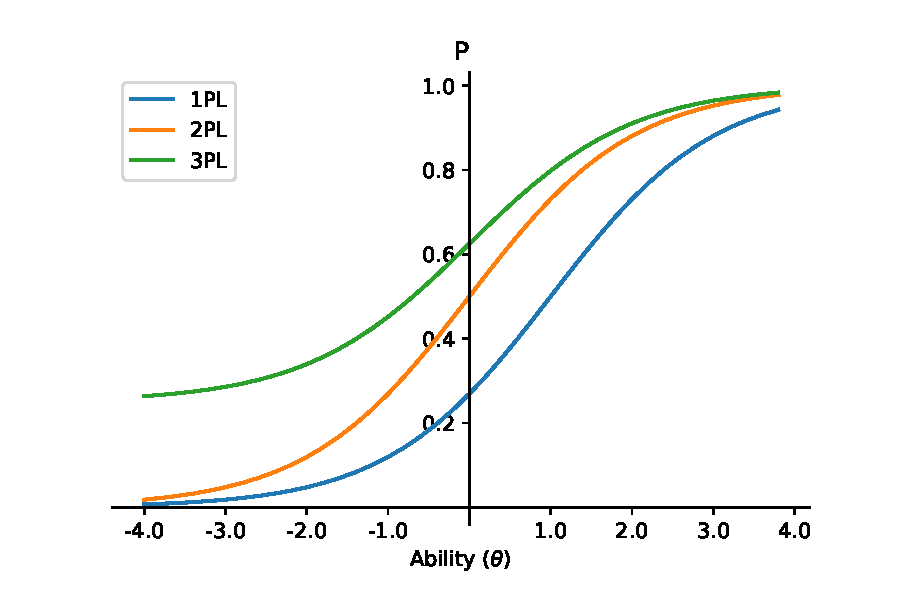
\includegraphics[scale=0.5]{figs/ICC_plots.pdf}
        \end{center}
        \caption{Một ví dụ về chèn hình ảnh.}
        \label{icc_plot}
    \end{figure}
\end{center}

\section{Chèn bảng}

\begin{center}
    \begin{table}
        \centering
        \caption{Ví dụ về tạo bảng trong \LaTeX. Tham khảo: \url{https://en.wikibooks.org/wiki/LaTeX/Tables}.}
        \begin{tabular}{ |l|l|l| }
            \hline
            \multicolumn{3}{ |c| }{Danh sách U23 Việt Nam tại Sea Games 31} \\
            \hline
            Thủ môn                   & GK & Nguyễn Văn Toản                \\ \hline
            \multirow{4}{*}{Hậu vệ}   & LB & Phan Tuấn Tài                  \\
                                      & DC & Bùi Hoàng Việt Anh             \\
                                      & DC & Lê Văn Đô                      \\
                                      & RB & Lê Văn Xuân                    \\ \hline
            \multirow{3}{*}{Tiền vệ}  & MC & Đỗ Hùng Dũng                   \\
                                      & MC & Nguyễn Hoàng Đức               \\
                                      & MC & Dụng Quang Nho                 \\ \hline

            \multirow{2}{*}{Tiền đạo} & ST & Nhâm Mạnh Dũng                 \\
                                      & ST & Nguyễn Văn Tùng                \\
                                      & FW & Nguyễn Tiến Linh               \\
            \hline
        \end{tabular}

    \end{table}
\end{center}

\section{Chèn công thức toán học}

Công thức \ref{eq:InterTweetInteraction} thể hiện mức độ tương tác giữa hai tập $T_{j}^{P}$ và $T_{k}^{P}$.

\begin{align}
    S_{j,k}^{P}=\frac{\sum_{t_{m}^{P}\in T_{j}^{P}}\sum_{t_{n}^{P}\in T_{k}^{P}}r\left(t_{m}^{P},t_{n}^{P}\right)}{|T_{j}^{P}||T_{k}^{P}|}\label{eq:InterTweetInteraction}
\end{align}

Để soạn thảo các công thức toán học được dễ dàng hơn, có thể sử dụng một phần mềm hỗ trợ nhập công thức theo dạng What You See Is What You Mean (WYSIWYM), chẳng hạn như \href{https://www.lyx.org/}{LyX}, sau đó copy LaTeX code vào file .tex (xem Hình \ref{lyx_example}), sẽ được kết quả như Công thức \ref{eq:ErrorFunction}.

\begin{center}
    \begin{figure}[h!]
        \begin{center}
            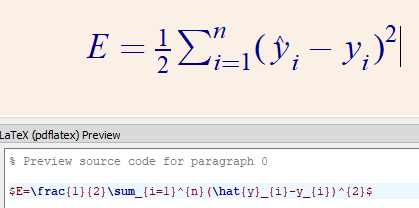
\includegraphics[scale=0.5]{figs/LyX.PNG}
        \end{center}
        \caption{Ví dụ cách soạn thảo công thức bằng LyX và copy sang file .tex.}
        \label{lyx_example}
    \end{figure}
\end{center}

\begin{align}
    E=\frac{1}{2}\sum_{i=1}^{n}(\hat{y}_{i}-y_{i})^{2}
    \label{eq:ErrorFunction}
\end{align}



\section{Chèn mã nguồn}
Có thể sử dụng package minted để chèn mã nguồn vào báo cáo. Có thể chèn mã nguồn trực tiếp hoặc từ file có sẵn.

\noindent\textbf{Ví dụ 1:} Chèn mã nguồn trực tiếp.
\lstset{language=Python}
\begin{lstlisting}
# Hello world program in Python
import math
def solve(a, b, c):
    if a == 0:
        if b != 0:
            return -c/b
        else:
            return "Phuong trinh vo nghiem hoac vo so nghiem"
    else:
        delta = b*b - 4*a*c
        if delta < 0:
            return "Phuong trinh vo nghiem"
        else:
            x1 = (-b + math.sqrt(delta)) / (2*a)
            x2 = (-b - math.sqrt(delta)) / (2*a)
            return x1, x2

print(solve(1, 2, 1))
\end{lstlisting}

\noindent\textbf{Ví dụ 2:} Chèn mã nguồn từ file. Đoạn mã nguồn sau đây được chèn từ file \path{code/XulyFileText.cpp}

\lstinputlisting[language=c++]{code/XulyFileText.cpp}

\section{Biểu diễn giải thuật}
\begin{algorithm}[H]
    \SetAlgoLined
    \KwIn{Hệ số $a$, $b$, và $c$ của phương trình bậc hai $ax^2 + bx + c = 0$}
    \KwOut{Nghiệm của phương trình}
    \If{$a = 0$}{
        \eIf{$b \neq 0$}{
            \Return{$x = -c/b$}\;
        }{
            \Return{Phương trình vô nghiệm hoặc vô số nghiệm}\;
        }
    }
    \Else{
        \textbf{Calculate} $\Delta = b^2 - 4ac$\;
        \eIf{$\Delta < 0$}{
            \Return{Phương trình vô nghiệm}\;
        }{
            \textbf{Calculate} $x1 = (-b + \sqrt{\Delta}) / (2a)$\;
            \textbf{Calculate} $x2 = (-b - \sqrt{\Delta}) / (2a)$\;
            \Return{$x1, x2$}\;
        }
    }
    \caption{Giải thuật giải phương trình bậc hai}
\end{algorithm}



\section{Chèn chú thích vào cuối trang (footnote)}
Khi cần chèn một dòng chú thích vào cuối trang, sử dụng lệnh \textbf{footnote}\footnote{Đây là dòng chú thích}.




\section{Chèn tài liệu tham khảo}

Có thể chèn tài liệu tham khảo vào báo cáo bằng cách sử dụng lệnh \textbf{cite} \cite{DBLP:journals/corr/abs-1908-10084}.
VD: \cite{DBLP:journals/corr/abs-1908-10084}.

VD2: \cite{van2010documentation, Gu_recognitionusing}.

% \input{chapter/chapter3-kienthucnentang.tex}
% \input{chapter/chapter4-huongtiepcan.tex}
% \input{chapter/chapter5-ketquadatduoc.tex}
% \input{chapter/chapter6-thaoluan.tex}

%bibliography{refs}{}
%bibliographystyle{plain}
%-	Danh mục TL tham khảo
%-	Phụ lục (nếu có)
\begin{thebibliography}{99}

	\bibitem{9direction}
	Chi Zhang, Rui Yao, Jinpeng Cai
	\textit{Efficient Eye Typing with 9 direction Gaze Estimation}.

	\bibitem{appearance}
	Xucong Zhang, Yusuke Sugano, Mario Fritz, Andreas Bulling
	\textit{Appearance-Based Gaze Estimation in the Wild}.


	\bibitem{eyeShapeRegistrationAndGazeEstimation}
	University of Cambridge, United Kingdom- Rendering of Eyes for Eye-Shape Registration and Gaze Estimation eww23 iccv2015
	\\\url{https://www.cv-foundation.org/openaccess/content_iccv_2015/papers/Wood_Rendering_of_Eyes_ICCV_2015_paper.pdf}

	\bibitem{Learninganappearancebasedgazeestimator}
	University of Cambridge and Carnegie Mellon University and Max Planck Institute for Informatics, Learning an appearance-based gaze estimator from one million synthesised images
	\\\url{https://www.d2.mpi-inf.mpg.de/content/learning-appearance-based-gaze-estimator-one-million-synthesised-images}

	\bibitem{AReviewandAnalysisofEyeGazeEstimation}
	Anuradha Kar and Peter M. Corcoran, A Review and Analysis of Eye-Gaze Estimation Systems Algorithms and Performance Evaluation Methods in Consumer Platforms
	\\\url{https://www.semanticscholar.org/paper/A-Review-and-Analysis-of-Eye-Gaze-Estimation-and-in-Kar-Corcoran/ae0a0ee1c6e2adcddffebf9b0e429a25b7d9c0e1}


	\bibitem{tangconv}
	\url{https://developer.apple.com/library/content/documentation/Performance/Conceptual/vImage/ConvolutionOperations/ConvolutionOperations.html}

	\bibitem{lenet5}
	Y. Lecun, L.Boutou, and Y.Bengio, Gradient-based learning applied to document recognition, Proceedings of the IEEE, vol. 88, no. 11, pp. 2278 – 2324, Nov. 1998.

	\bibitem{maxpool}
	Denny Britz,
	\url{http://www.wildml.com/2015/11/understanding-convolutional-neural-networks-for-nlp/}

	\bibitem{cnn}
	Brandon Rohrer, \url{http://brohrer.github.io/how_convolutional_neural_networks_work.html}

	\bibitem{fullconnect}
	Trần Thế Anh,
	\url{http://labs.septeni-technology.jp/technote/ml-20-convolution-neural-network-part-3/}
	\bibitem{ptha}
	Lương Quốc An,
	\url{http://nhiethuyettre.net/mang-no-ron-tich-chap-convolutional-neural-network/}

	\bibitem{inception}
	\url{https://leonardoaraujosantos.gitbooks.io/artificial-inteligence/content/googlenet.html}

	\bibitem{softmax}
	Giáo trình Mạng neural, Tác giả: Phan Văn Hiền – Trường Đại học Bách khoa Đà Nẵng, 2013

	\bibitem{alexnet} Aarshay Jain,
	\url{https://www.analyticsvidhya.com/blog/2016/04/deep-learning-computer-vision-introduction-convolution-neural-networks/}
	\bibitem{dataset}
	\url{https://www.mpi-inf.mpg.de/departments/computer-vision-and-multimodal-computing/research/gaze-based-human-computer-interaction/its-written-all-over-your-face-full-face-appearance-based-gaze-estimation/}

	\bibitem{}
	\url{https://www.tensorflow.org/versions/r0.12/get_started/basic_usage}

	\bibitem{gglenet}
	Christian Szegedy, Wei Liu, Yangqing Jia, Pierre Sermanet, Scott Reed, Dragomir Anguelov, Dumitru Erhan, Vincent Vanhouke, Andrew Rabinovich. \textit{Going deeper with convolutions}

	\bibitem{renset}
	Kaiming He, Xiangyu Zhang, Shaoqing Ren, Jian Sun \textit{Deep Residual Learning for Image Recognition}

	\bibitem{tensor} Trần Thế Anh,
	\url{http://labs.septeni-technology.jp/technote/ml-18-convolution-neural-network-part-1/}

	\bibitem{mangcnn}
	\url{https://www.kernix.com/blog/a-toy-convolutional-neural-network-for-image-classification-with-keras_p14}
	\bibitem{GazeCaptureEyeTracking}
	Kyle Krafka- Aditya Khosla- Petr Kellnhofer- Harini Kannan- Suchendra Bhandarkar- Wojciech Matusik- Antonio Torralba, Eye Tracking for Everyone
	\url{http://gazecapture.csail.mit.edu/}

	\bibitem{GazeCapturegit}
	Kyle Krafka and Aditya Khosla and Petr Kellnhofer and Harini Kannan and Suchendra Bhandarkar and Wojciech Matusik and Antonio Torralba, Eye Tracking for Everyone Code Dataset and Models
	\url{https://github.com/CSAILVision/GazeCapture}

	\bibitem{eyetrackingapplication}
	\url{https://medium.com/@taolu_99738/developing-of-eye-tracking-application-for-smartphone-b875c50ee0c3}

\end{thebibliography}
\end{document}